\subsection{MLCommons Science - Earthquake}
{{\footnotesize
\noindent MLCommons Science assembles benchmark tasks with datasets, targets, and implementations across earthquake forecasting, satellite imagery, drug screening, electron microscopy, and CFD to drive scientific ML reproducibility.


\begin{description}[labelwidth=4cm, labelsep=1em, leftmargin=4cm, itemsep=0.1em, parsep=0em]
  \item[date:] 2023-06-01
  \item[version:] v1.0
  \item[last\_updated:] 2023-06
  \item[expired:] no
  \item[valid:] yes
  \item[valid\_date:] 2023-06-01
  \item[url:] \href{https://github.com/mlcommons/science}{https://github.com/mlcommons/science}
  \item[doi:] 10.1007/978-3-031-23220-6\_4
  \item[domain:]
    - Climate \& Earth Science
  \item[focus:] AI benchmarks for scientific applications including time-series, imaging, and simulation
  \item[keywords:]
    - science AI
    - benchmark
    - MLCommons
    - HPC
  \item[licensing:] Apache License 2.0
  \item[task\_types:]
    - Time-series analysis
    - Image classification
    - Simulation surrogate modeling
  \item[ai\_capability\_measured:]
    - Inference accuracy
    - simulation speed-up
    - generalization
  \item[metrics:]
    - MAE
    - Accuracy
    - Speedup vs simulation
  \item[models:]
    - CNN
    - GNN
    - Transformer
  \item[ml\_motif:]
    - Sequence Prediction/Forecasting
  \item[type:] Framework
  \item[ml\_task:]
    - NA
  \item[solutions:] 0
  \item[notes:] Joint effort under Apache-2.0 license.

  \item[contact.name:] MLCommons Science Working Group
  \item[contact.email:] science-chairs@mlcommons.org
  \item[datasets.links.name:] CANDLE UNO
  \item[datasets.links.url:] \href{https://github.com/mlcommons/science/tree/main/benchmarks/uno\#data-description}{https://github.com/mlcommons/science/tree/main/benchmarks/uno\#data-description}
  \item[results.links.name:] ChatGPT LLM
  \item[fair.reproducible:] Yes
  \item[fair.benchmark\_ready:] Yes
  \item[id:] mlcommons\_science\_-\_earthquake
  \item[Citations:] \cite{10.1007/978-3-031-23220-6_4}
\end{description}

{\bf Ratings:} ~ \\

\begin{tabular}{p{0.15\textwidth} p{0.07\textwidth} p{0.7\textwidth}}
\hline
Rating & Value & Reason \\
\hline
dataset & 5 & Public scientific datasets are used with defined splits. At least 4 FAIR principles
are followed.
 \\
documentation & 5 & Thorough documentation exists covering the task, background, motivation, evaluation
criteria, and includes a supporting paper.
 \\
metrics & 5 & Clearly defined metrics such as accuracy, training time, and GPU utilization are
used. These metrics are explained and effectively capture solution performance.
 \\
reference\_solution & 5 & A reference implementation is available, well-documented, trainable/open, and includes
full metric evaluation and software/hardware details.
 \\
software & 5 & Actively maintained GitHub repository available at https://github.com/mlcommons/science
with implementations, scripts, and reproducibility support.
 \\
specification & 5 & All five specification aspects are covered: system constraints, task, dataset format,
benchmark inputs, and outputs.
 \\
\hline
\end{tabular}

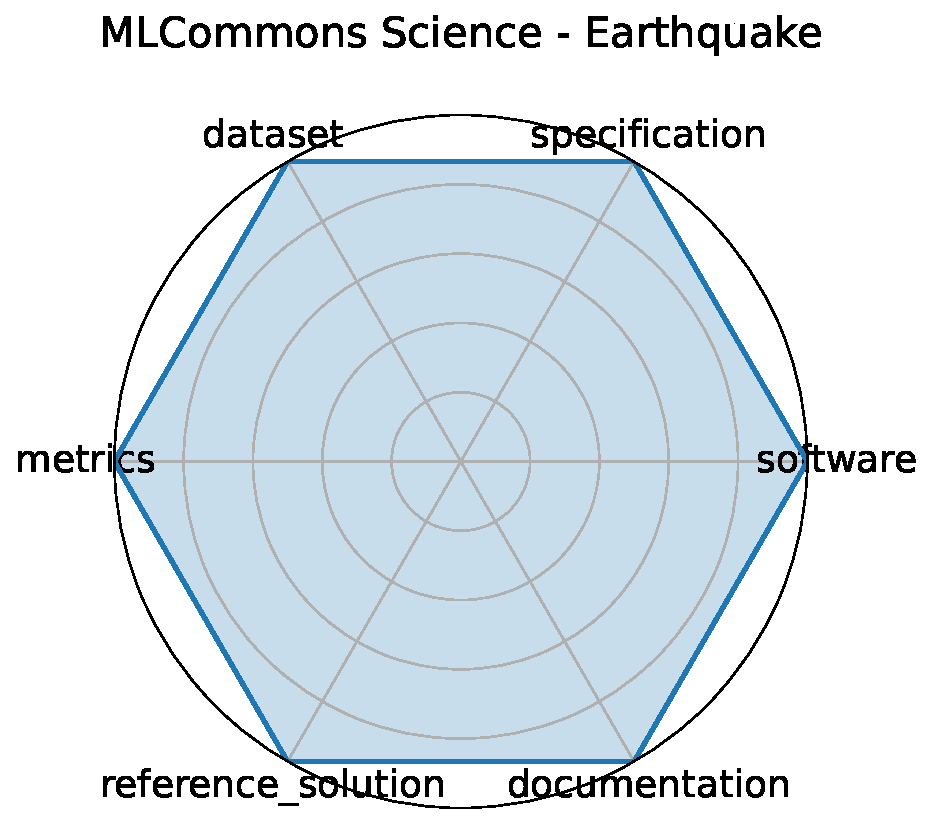
\includegraphics[width=0.2\textwidth]{mlcommons_science_-_earthquake_radar.pdf}
}}
\clearpage